\documentclass[twocolumn]{article}

\usepackage{arxiv}

\usepackage[utf8]{inputenc}
\usepackage[T1]{fontenc}
\usepackage{hyperref}
\usepackage{url}
\usepackage{booktabs}
\usepackage{amsfonts}
\usepackage{amsmath}
\usepackage{nicefrac}
\usepackage{microtype}
\usepackage{graphicx}
\usepackage{natbib}
\usepackage{doi}

\graphicspath{{figures/}}

\title{Internal Excellence, External Collapse: A Rigorous Audit of a\\ Knowledge-Distilled Cervical Cytology Classifier}

\renewcommand{\shorttitle}{Internal Excellence, External Collapse}

\author{Cervical Cytology Pipeline}

\hypersetup{
pdftitle={Internal Excellence, External Collapse},
pdfsubject={q-bio.QM, cs.CV},
pdfkeywords={cervical cytology, knowledge distillation, domain shift, calibration, SIPaKMeD},
}

\begin{document}

\twocolumn[
\begin{@twocolumnfalse}
\maketitle
\begin{abstract}
We audit a two-stage EfficientNet-B4 teacher knowledge-distilled into an EfficientNet-B0 student
for five-class cervical-cell classification on \textbf{SIPaKMeD}. In-distribution the distilled
student is excellent---$96.6\%$ accuracy, $0.967$ macro-$F_1$, $0.998$ one-vs-rest AUROC, and an
expected calibration error (ECE) of only $0.015$---and it surpasses its own teacher ($94.3\%$).
Grad-CAM confirms the model attends to nuclear/cellular structure. Yet under a binary
normal/abnormal collapse the same model \emph{collapses out-of-distribution}: $63.9\%$ on Herlev,
$60.5\%$ on HiCervix and $53.2\%$ on APACC, with AUROCs of $0.73$, $0.59$ and $0.53$. We diagnose
the cause in detail and show it is \emph{not} a labelling artefact: the predicted
$P(\mathrm{abnormal})$ ranks abnormal above normal cells in every dataset (positive separation,
AUROC$>0.5$). Instead the failure is (i) genuine domain-shift signal degradation that tracks slide
preparation similarity (conventional smear $\rightarrow$ liquid-based $\rightarrow$ auto-segmented
crops), and (ii) a per-domain shift of the decision score that makes the fixed $\tau{=}0.5$
operating point underperform even a majority-class baseline despite real ranking signal. The
internal number is itself optimistic because it is measured on a leaky random split. We conclude
that headline accuracy is a poor proxy for screening readiness, and that the remedies are
leakage-safe evaluation, stain/domain normalization and per-domain calibration---not relabelling.
\end{abstract}
\keywords{cervical cytology \and knowledge distillation \and domain shift \and calibration \and SIPaKMeD}
\bigskip
\end{@twocolumnfalse}
]

\section{Introduction}
Automated cervical-cytology screening is dominated by lightweight, edge-deployable models trained
and evaluated \emph{within a single dataset}, where reported accuracies routinely exceed $97\%$.
Our starting point is exactly such a model: an EfficientNet-B4 teacher~\citep{tan2019efficientnet}
distilled~\citep{hinton2015distilling} into an EfficientNet-B0 student on
SIPaKMeD~\citep{plissiti2018sipakmed}. This report asks a single question---\emph{does it
generalize?}---and answers it with an honest cross-dataset audit. We report the full
in-distribution performance, calibration and Grad-CAM explanations, then the cross-dataset results,
and finally a detailed diagnosis of why the model fails to transfer.

\section{Methods}
\textbf{Data.} SIPaKMeD provides $4{,}049$ cropped single cells in five cytomorphology classes
(Superficial-Intermediate, Parabasal, Metaplastic, Koilocytotic, Dyskeratotic). \textbf{Model.} The
B4 teacher is trained in two stages (frozen backbone, then fine-tuned), and a B0 student is trained
by distillation with the canonical temperature-scaled logit loss
$\mathcal{L}=\alpha\,\mathrm{CE}+(1-\alpha)\,T^2\,\mathrm{KL}\!\left(\sigma(z_t/T)\,\|\,\sigma(z_s/T)\right)$.
\textbf{Cross-dataset protocol.} The native label spaces of the external sets do not match
SIPaKMeD's five classes, so both the prediction and the ground truth are collapsed to a binary
normal/abnormal decision, scoring $P(\mathrm{abnormal})=\sigma(z)_{\text{Koilo}}+\sigma(z)_{\text{Dysk}}$
against a pre-registered threshold $\tau{=}0.5$. Glandular and indeterminate native classes have no
home in the squamous five-class space and are excluded (and the excluded fraction reported).

\section{In-distribution results}
\textbf{Training.} The teacher converges over $71$ epochs (30 frozen $+$ 41 fine-tuning,
early-stopped) and the student over $34$ epochs; Figure~\ref{fig:curves} shows smooth, non-overfit
train/validation curves.

\begin{figure}[t]
  \centering
  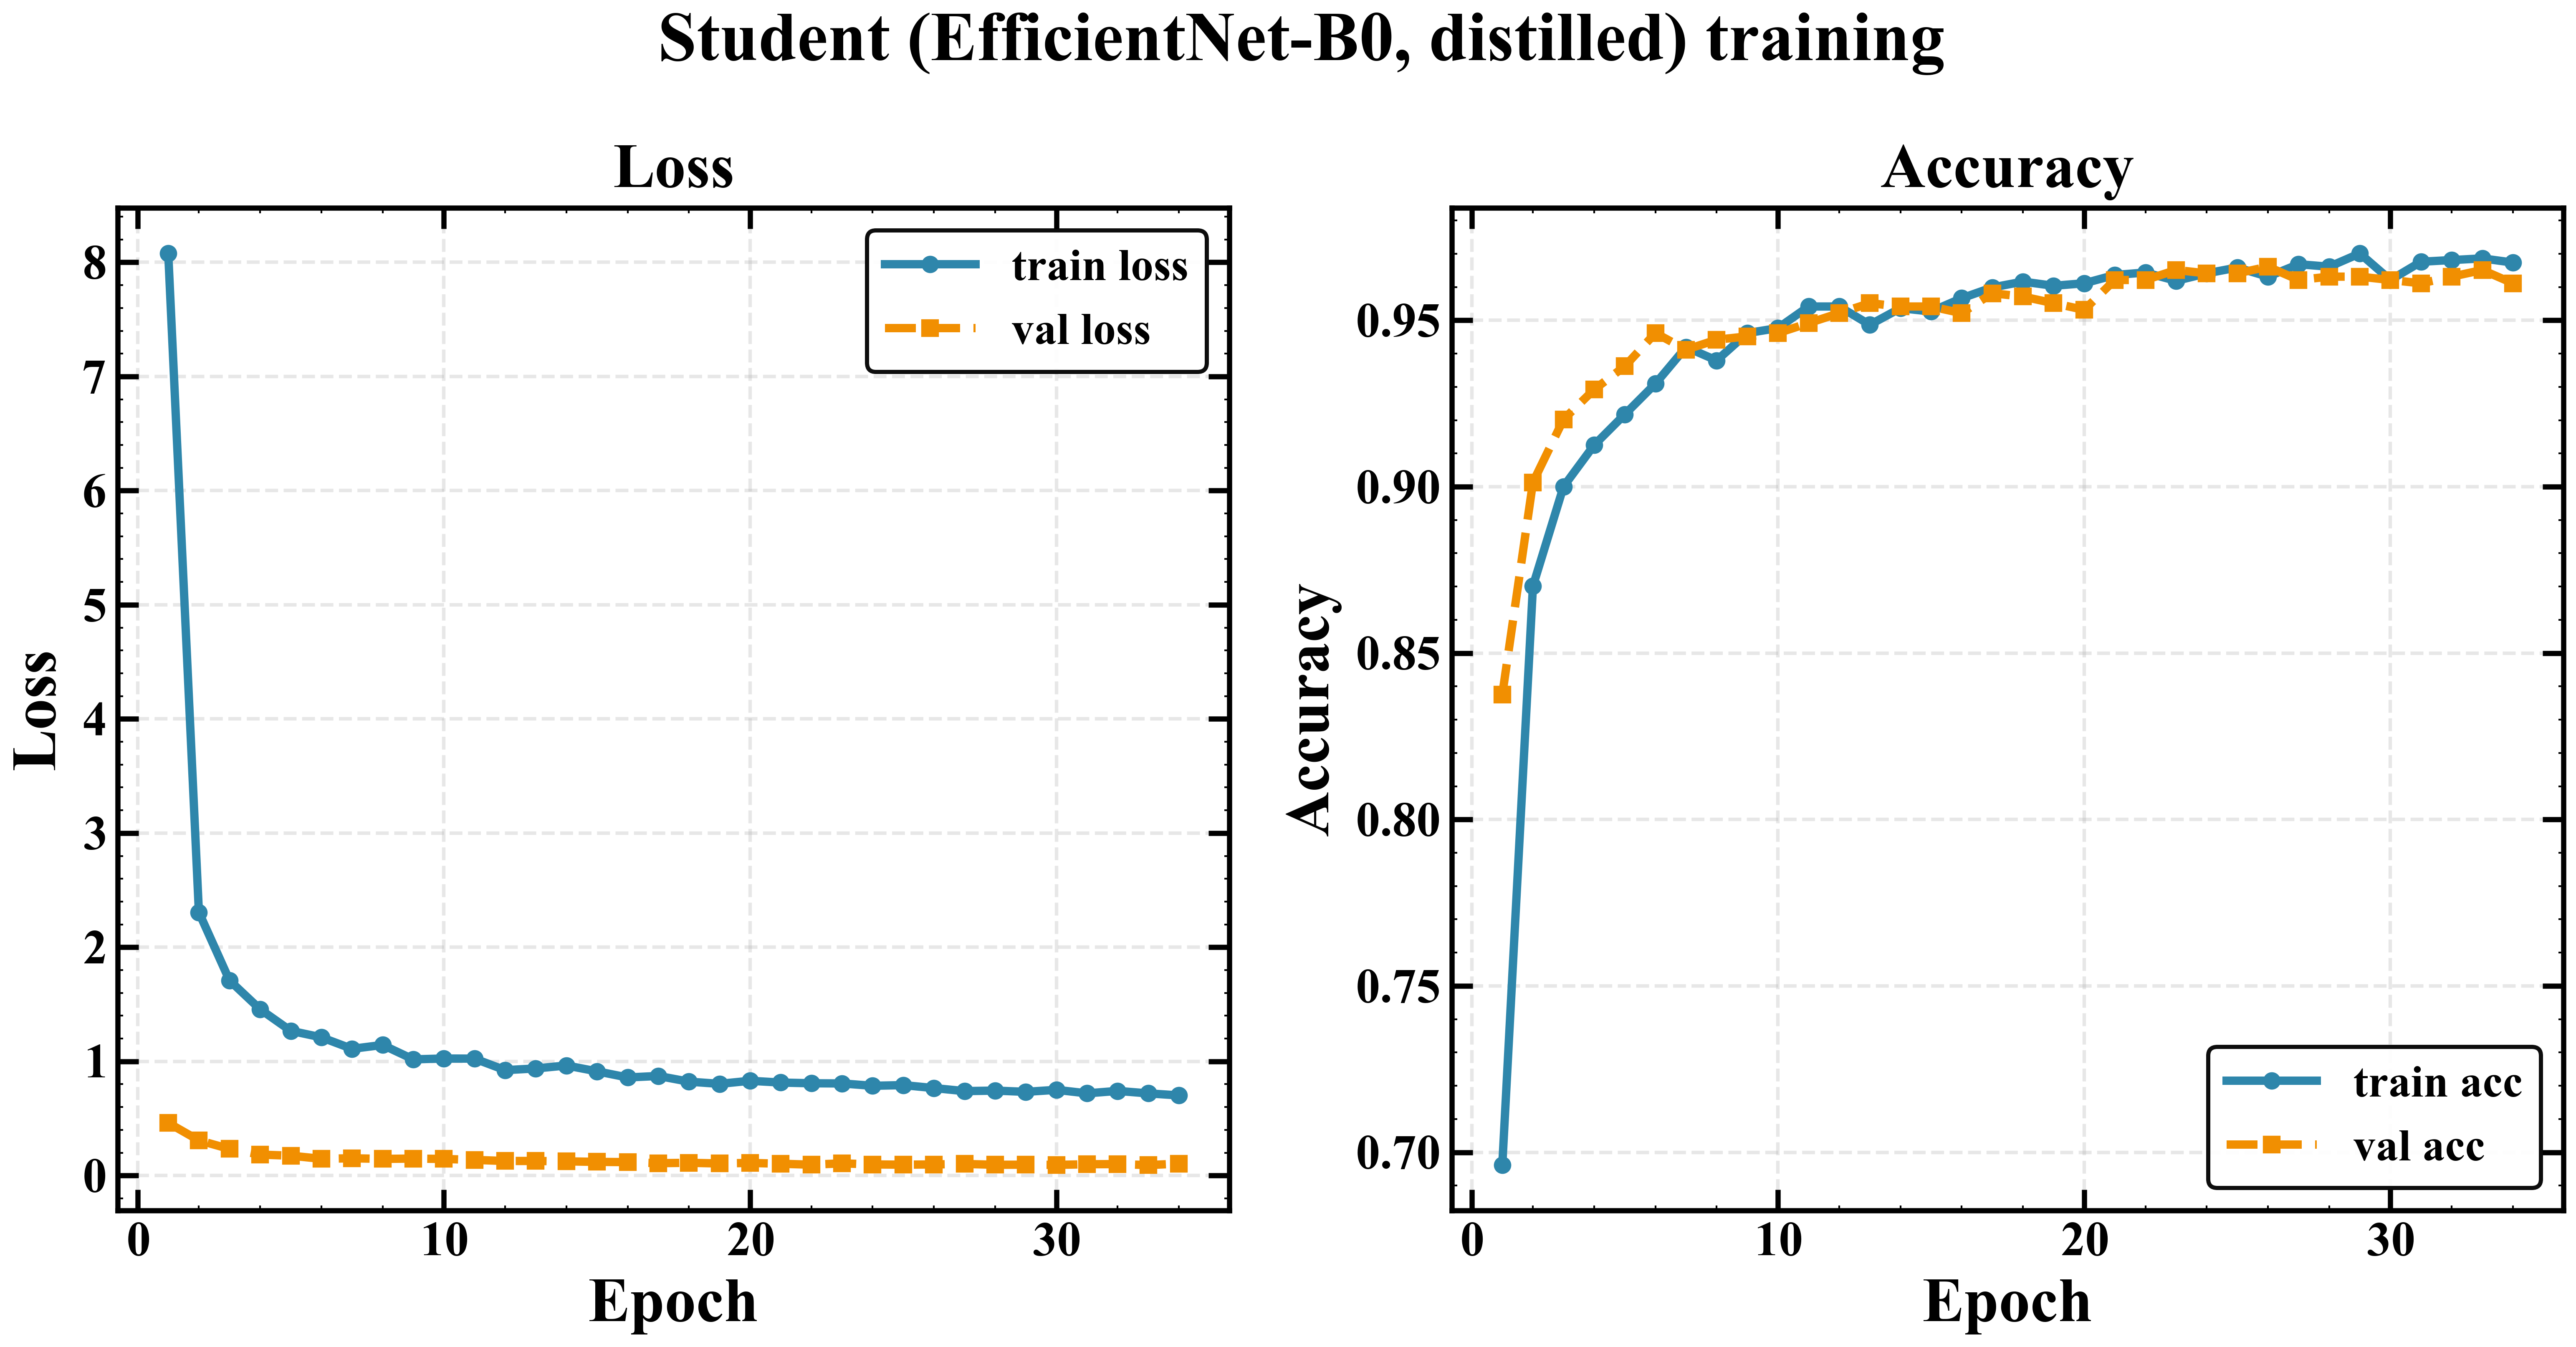
\includegraphics[width=\linewidth]{student_training_curves.png}
  \caption{Distilled B0 student training: train/validation loss and accuracy. Validation tracks
  training closely (no overfitting), converging to $\approx 96\%$ validation accuracy.}
  \label{fig:curves}
\end{figure}

\textbf{Classification.} Table~\ref{tab:indist} reports the five-class metrics. The distilled
student reaches $96.6\%$ accuracy and \emph{exceeds} its teacher on every metric---evidence that the
distillation signal is informative rather than inert. Per-class $F_1$ (student) is highest for
Superficial-Intermediate ($0.995$) and Parabasal ($0.994$) and lowest for Koilocytotic
($0.919$, recall $0.873$), the class most often confused with its neighbours
(Figure~\ref{fig:cm_student}).

\begin{table}[t]
  \caption{In-distribution five-class metrics (SIPaKMeD validation). The distilled student surpasses
  the teacher on all metrics and is well calibrated.}
  \label{tab:indist}
  \centering
  \small
  \begin{tabular}{lcc}
    \toprule
    Metric & Teacher (B4) & \textbf{Student (B0)} \\
    \midrule
    Accuracy           & 0.943 & \textbf{0.966} \\
    Balanced accuracy  & 0.946 & \textbf{0.968} \\
    Macro-$F_1$        & 0.945 & \textbf{0.967} \\
    Cohen's $\kappa$   & 0.929 & \textbf{0.958} \\
    AUROC (OvR)        & 0.996 & \textbf{0.998} \\
    ECE                & 0.013 & 0.015 \\
    \bottomrule
  \end{tabular}
\end{table}

\begin{figure}[t]
  \centering
  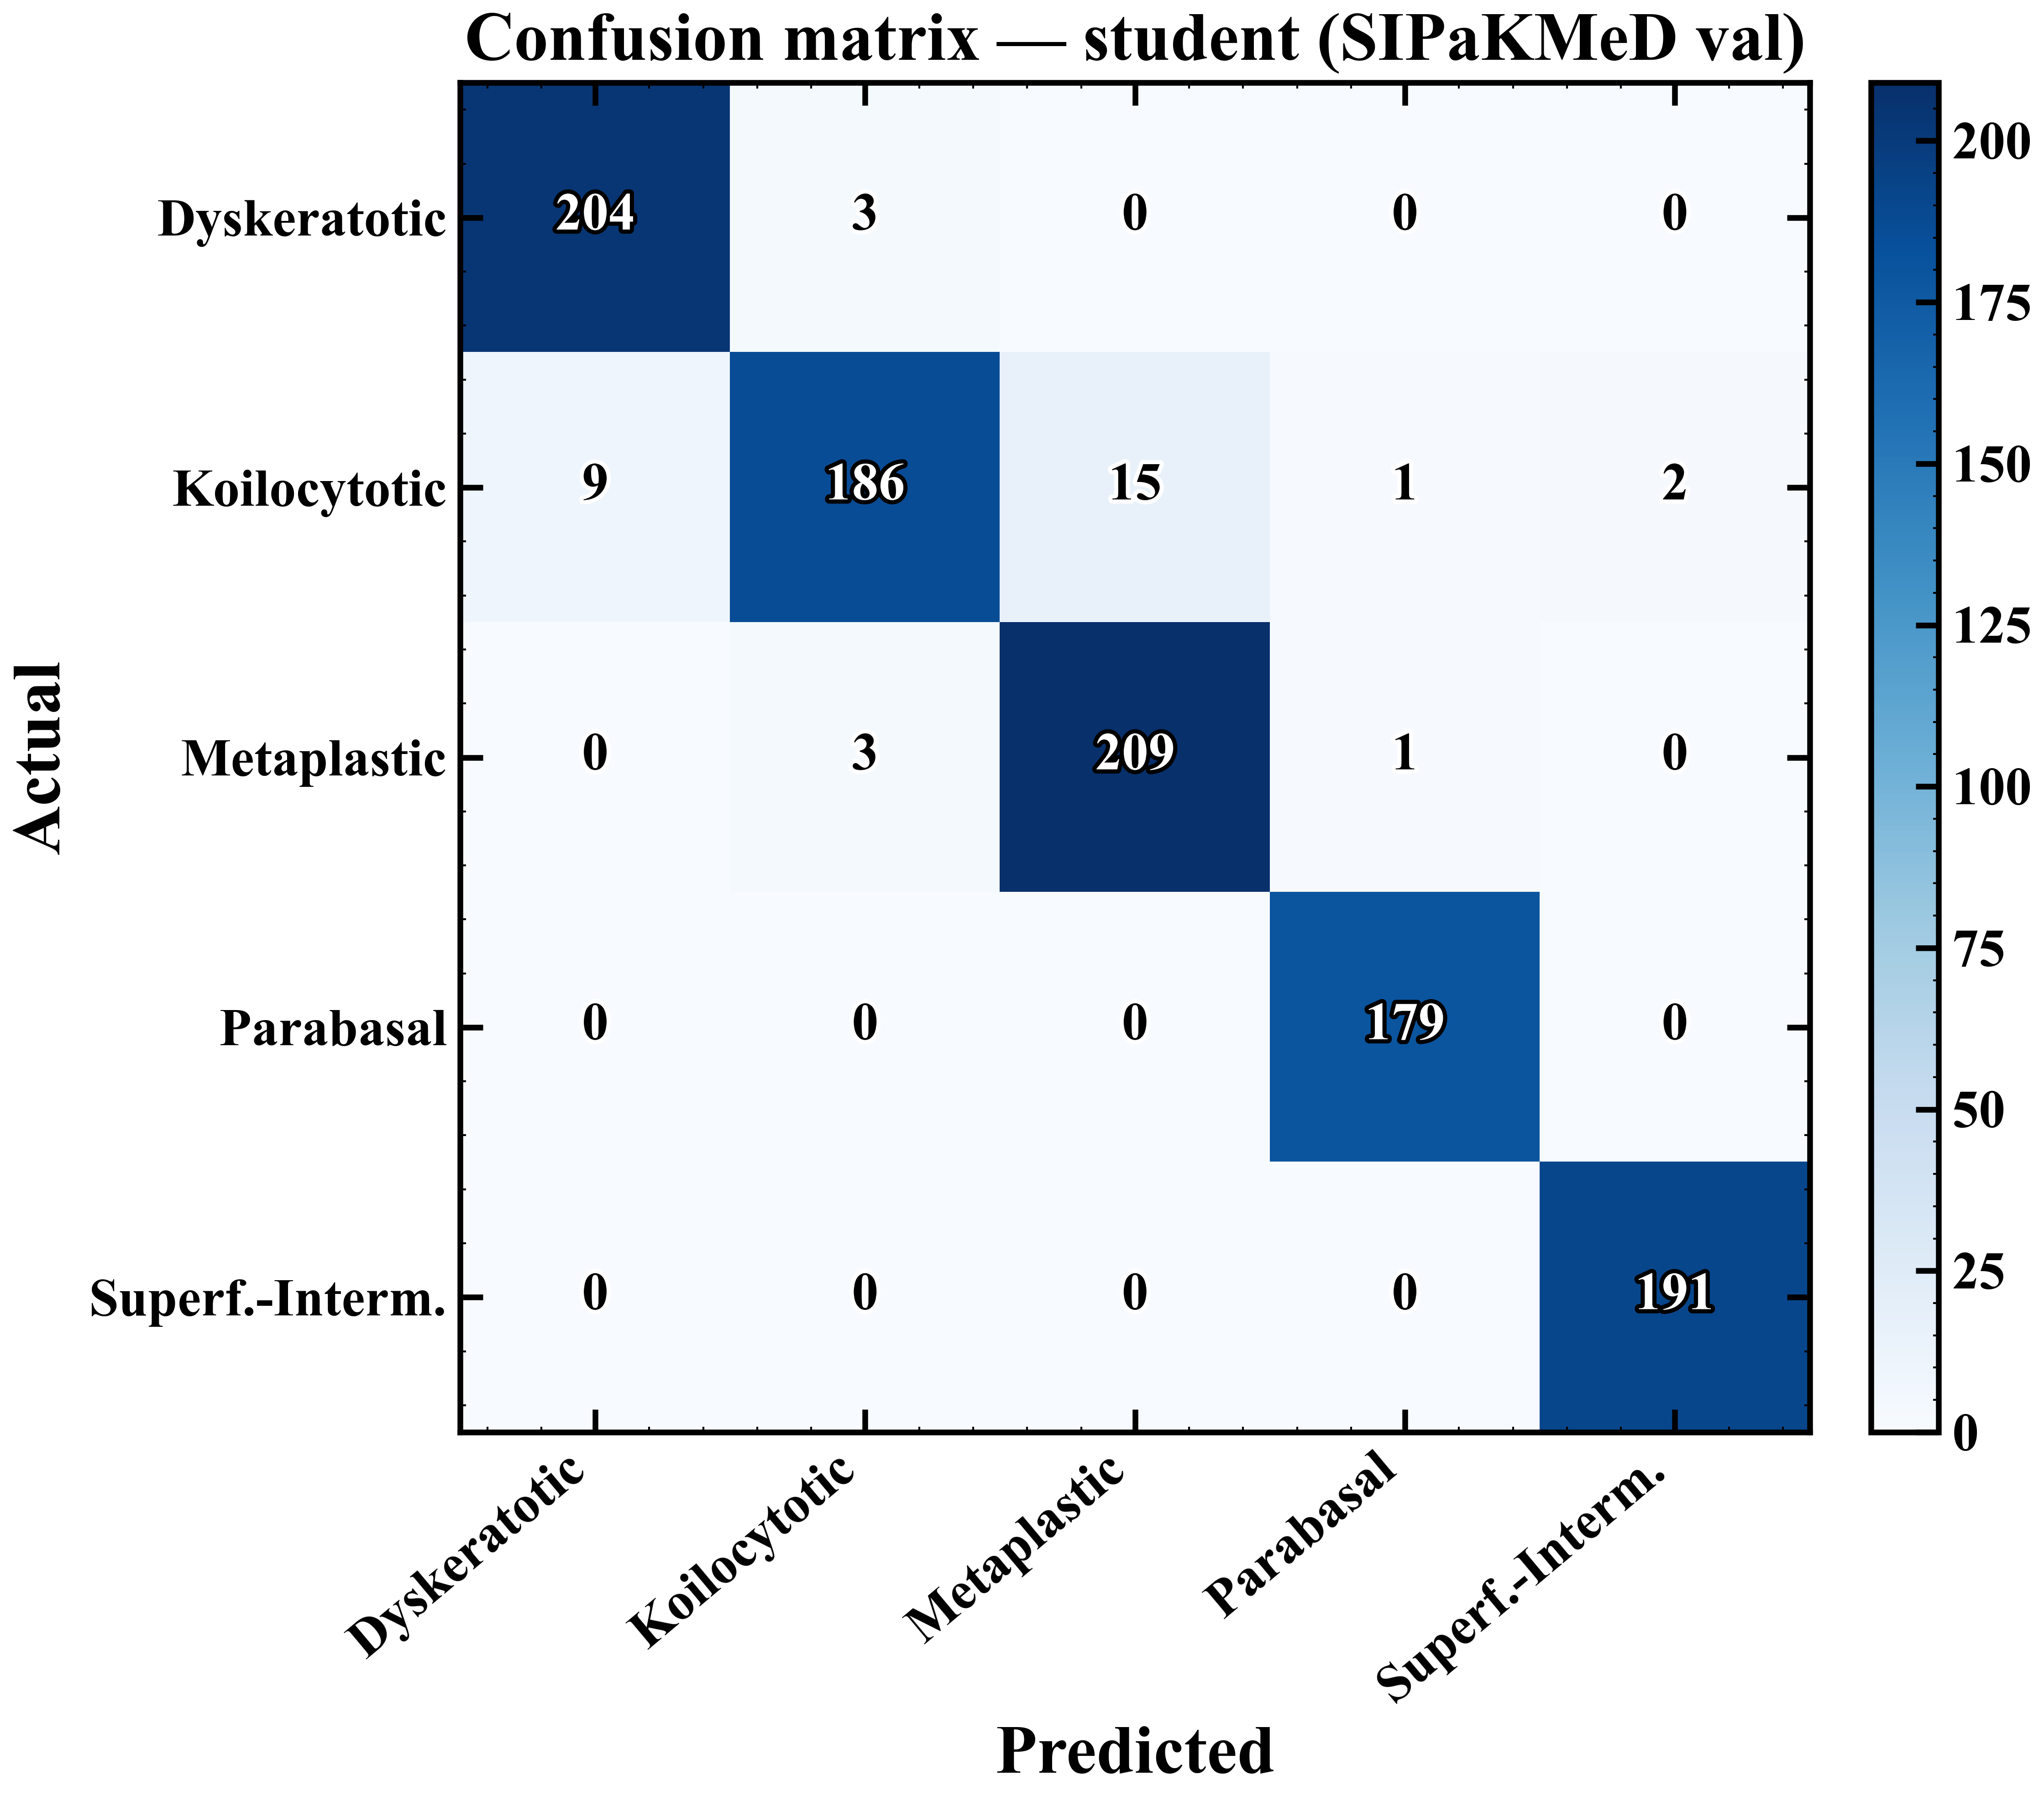
\includegraphics[width=\linewidth]{cm_student.png}
  \caption{Five-class confusion matrix (student). Errors concentrate on Koilocytotic, which is
  confused with the other abnormal/metaplastic classes.}
  \label{fig:cm_student}
\end{figure}

\textbf{Calibration.} Both models are well calibrated: ECE $=0.013$ (teacher) and $0.015$
(student). The reliability diagram (Figure~\ref{fig:reliability}) lies close to the identity,
meaning the in-distribution confidences are trustworthy---a property we show \emph{does not} survive
the domain shift.

\begin{figure}[t]
  \centering
  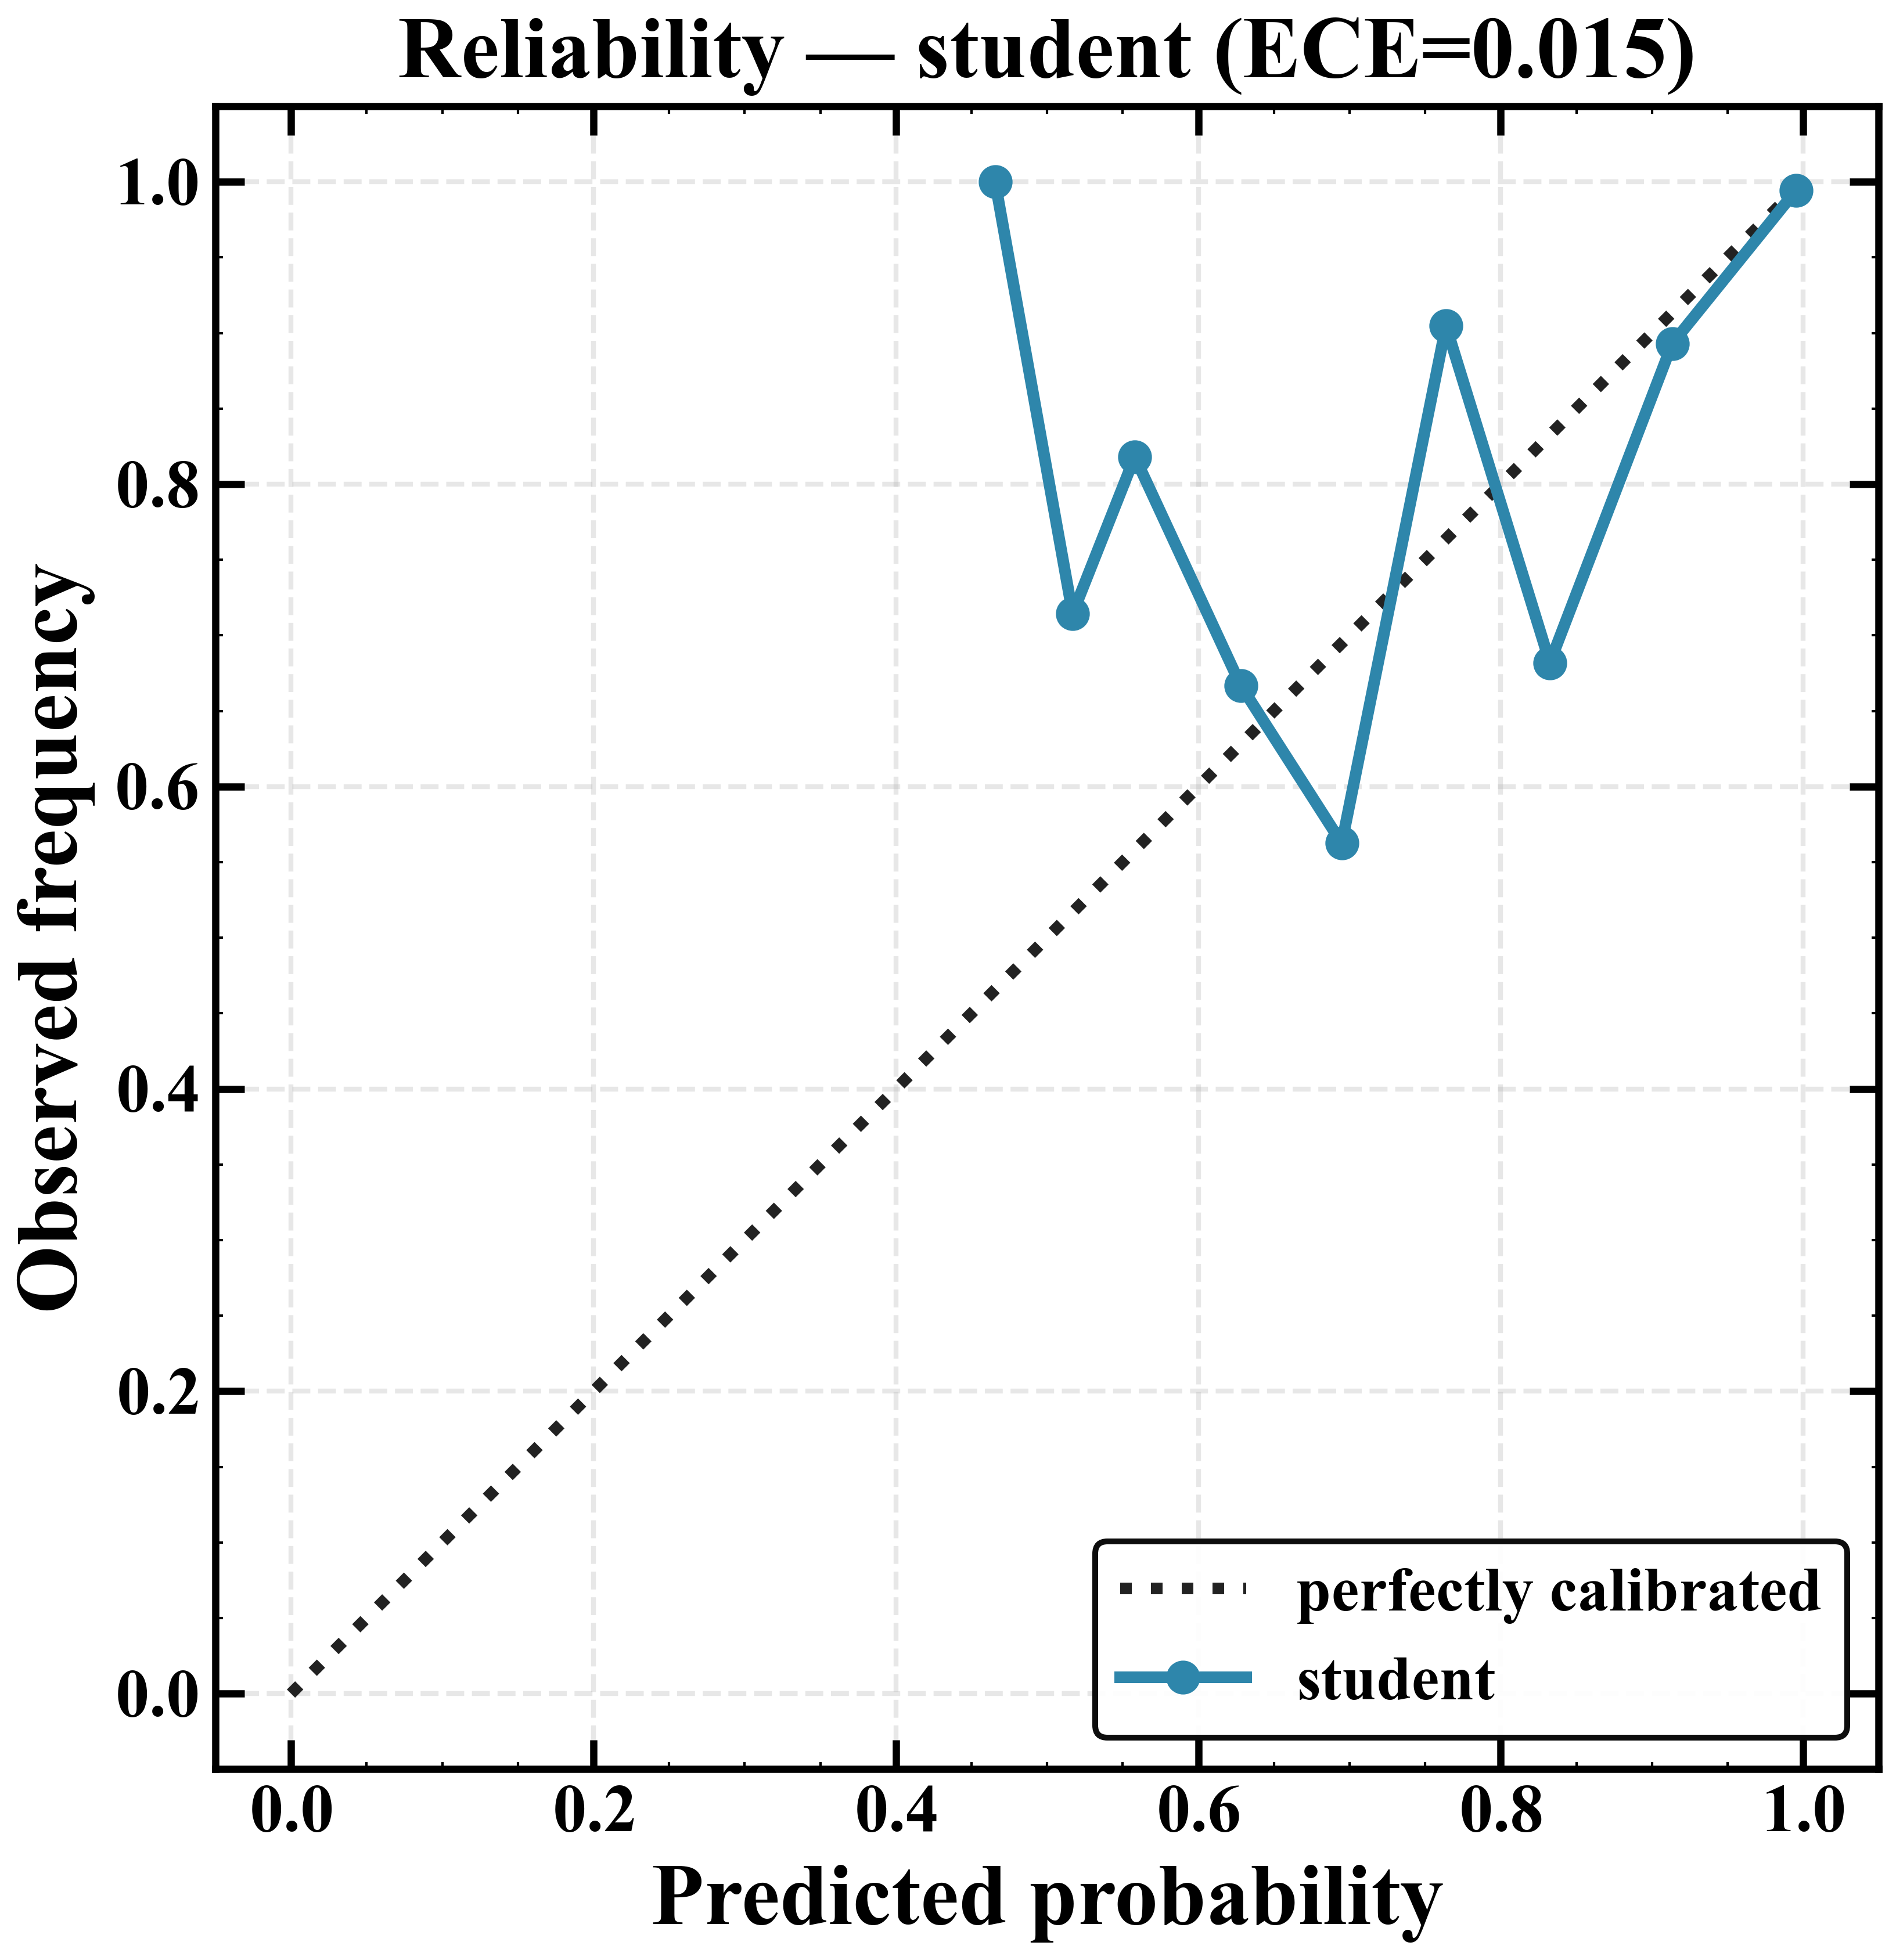
\includegraphics[width=\linewidth]{reliability_student.png}
  \caption{Reliability diagram (student, ECE $=0.015$). In-distribution confidence is well
  calibrated; bins lie close to the diagonal.}
  \label{fig:reliability}
\end{figure}

\section{Explainability}
Grad-CAM~\citep{selvaraju2017gradcam} over the student's final convolutional block
(Figure~\ref{fig:gradcam}) localizes the evidence to the nucleus and cell body for one
representative correctly-classified cell per class (confidences $0.97$--$1.00$). The attributions
are cytologically plausible, indicating the in-distribution decisions are driven by cell structure
rather than background artefacts.

\begin{figure*}[t]
  \centering
  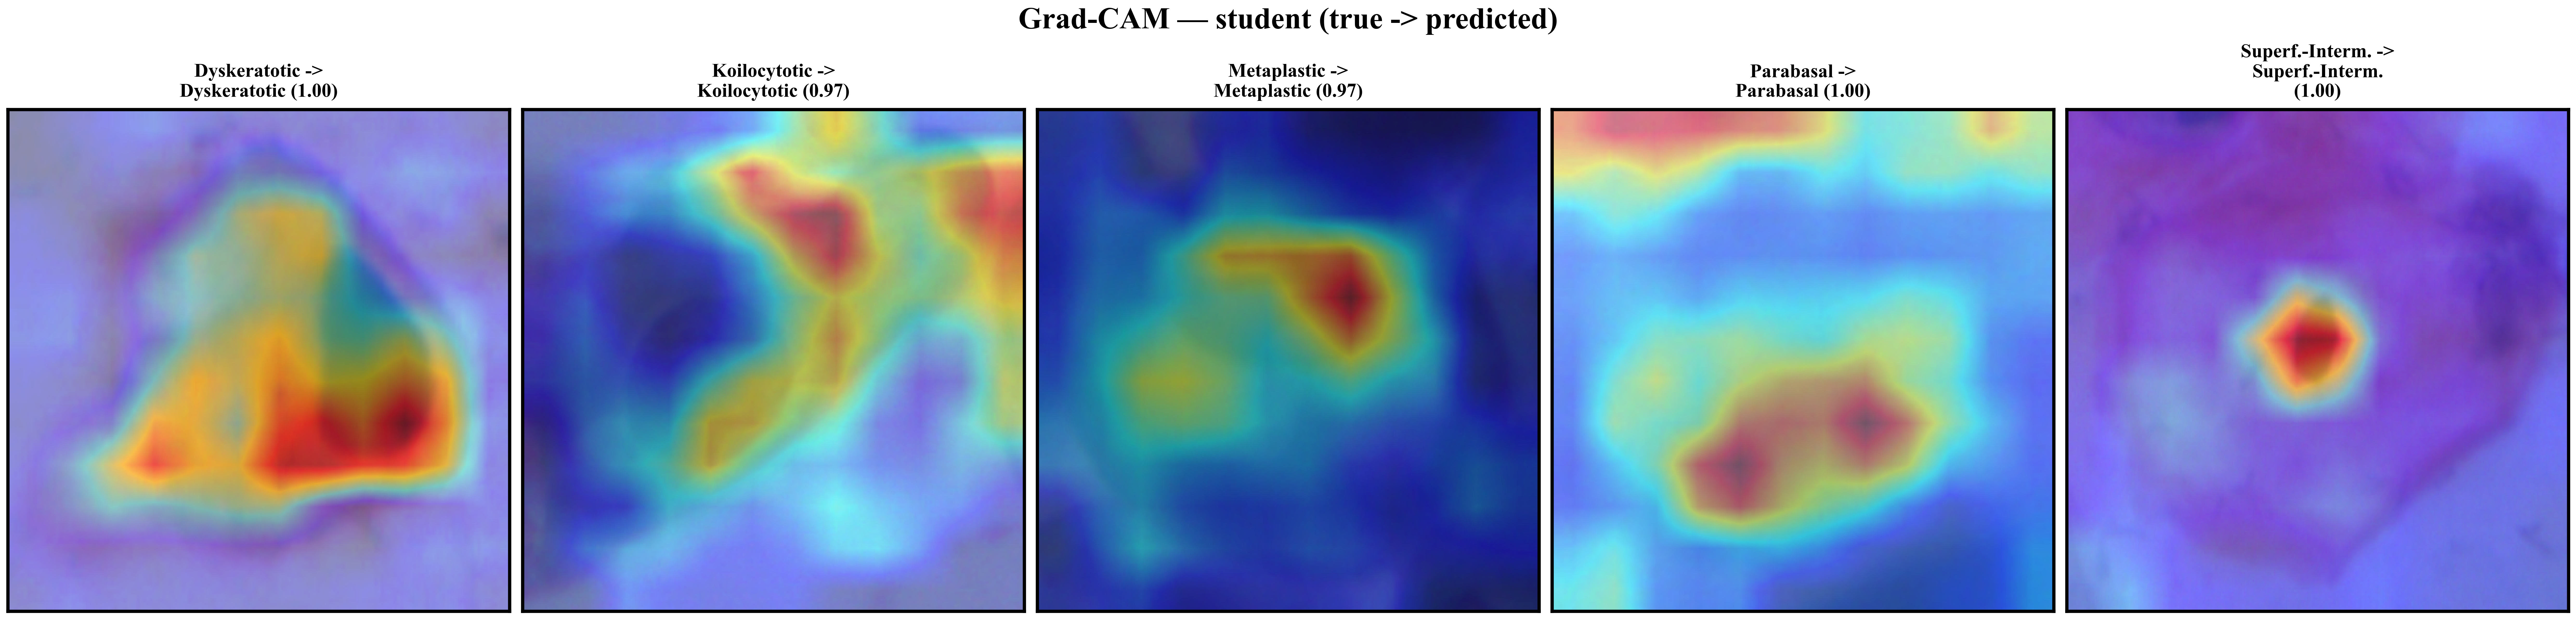
\includegraphics[width=\textwidth]{gradcam_student.png}
  \caption{Grad-CAM for the student, one representative cell per SIPaKMeD class (true
  $\rightarrow$ predicted, confidence). Heatmaps concentrate on nuclear/cellular regions.}
  \label{fig:gradcam}
\end{figure*}

\section{Cross-dataset generalization}
We evaluate the SIPaKMeD-trained student, unchanged, on three external single-cell Pap datasets at
the binary level. Table~\ref{tab:cross} and Figure~\ref{fig:cmcross} report the result: accuracy
falls from $96.6\%$ internally to $53$--$64\%$ externally, with AUROCs of $0.53$--$0.73$. Sensitivity
on HiCervix is only $0.39$---the model \emph{misses most abnormal cells} out of distribution.

\begin{table}[t]
  \caption{Cross-dataset binary (normal/abnormal) results for the student. $\Delta P$ is the
  separation between mean $P(\mathrm{abnormal})$ on true-abnormal vs.\ true-normal cells (positive
  $=$ correct ordering). Internal SIPaKMeD accuracy is $0.966$.}
  \label{tab:cross}
  \centering
  \small
  \begin{tabular}{lccccc}
    \toprule
    Dataset & $n$ & Acc & Sens & Spec & AUROC \\
    \midrule
    Herlev   & 917  & 0.639 & 0.625 & 0.678 & \textbf{0.728} \\
    HiCervix & 4823 & 0.605 & 0.386 & 0.738 & 0.594 \\
    APACC    & 1125 & 0.532 & 0.654 & 0.417 & 0.525 \\
    \bottomrule
  \end{tabular}
\end{table}

\begin{figure*}[t]
  \centering
  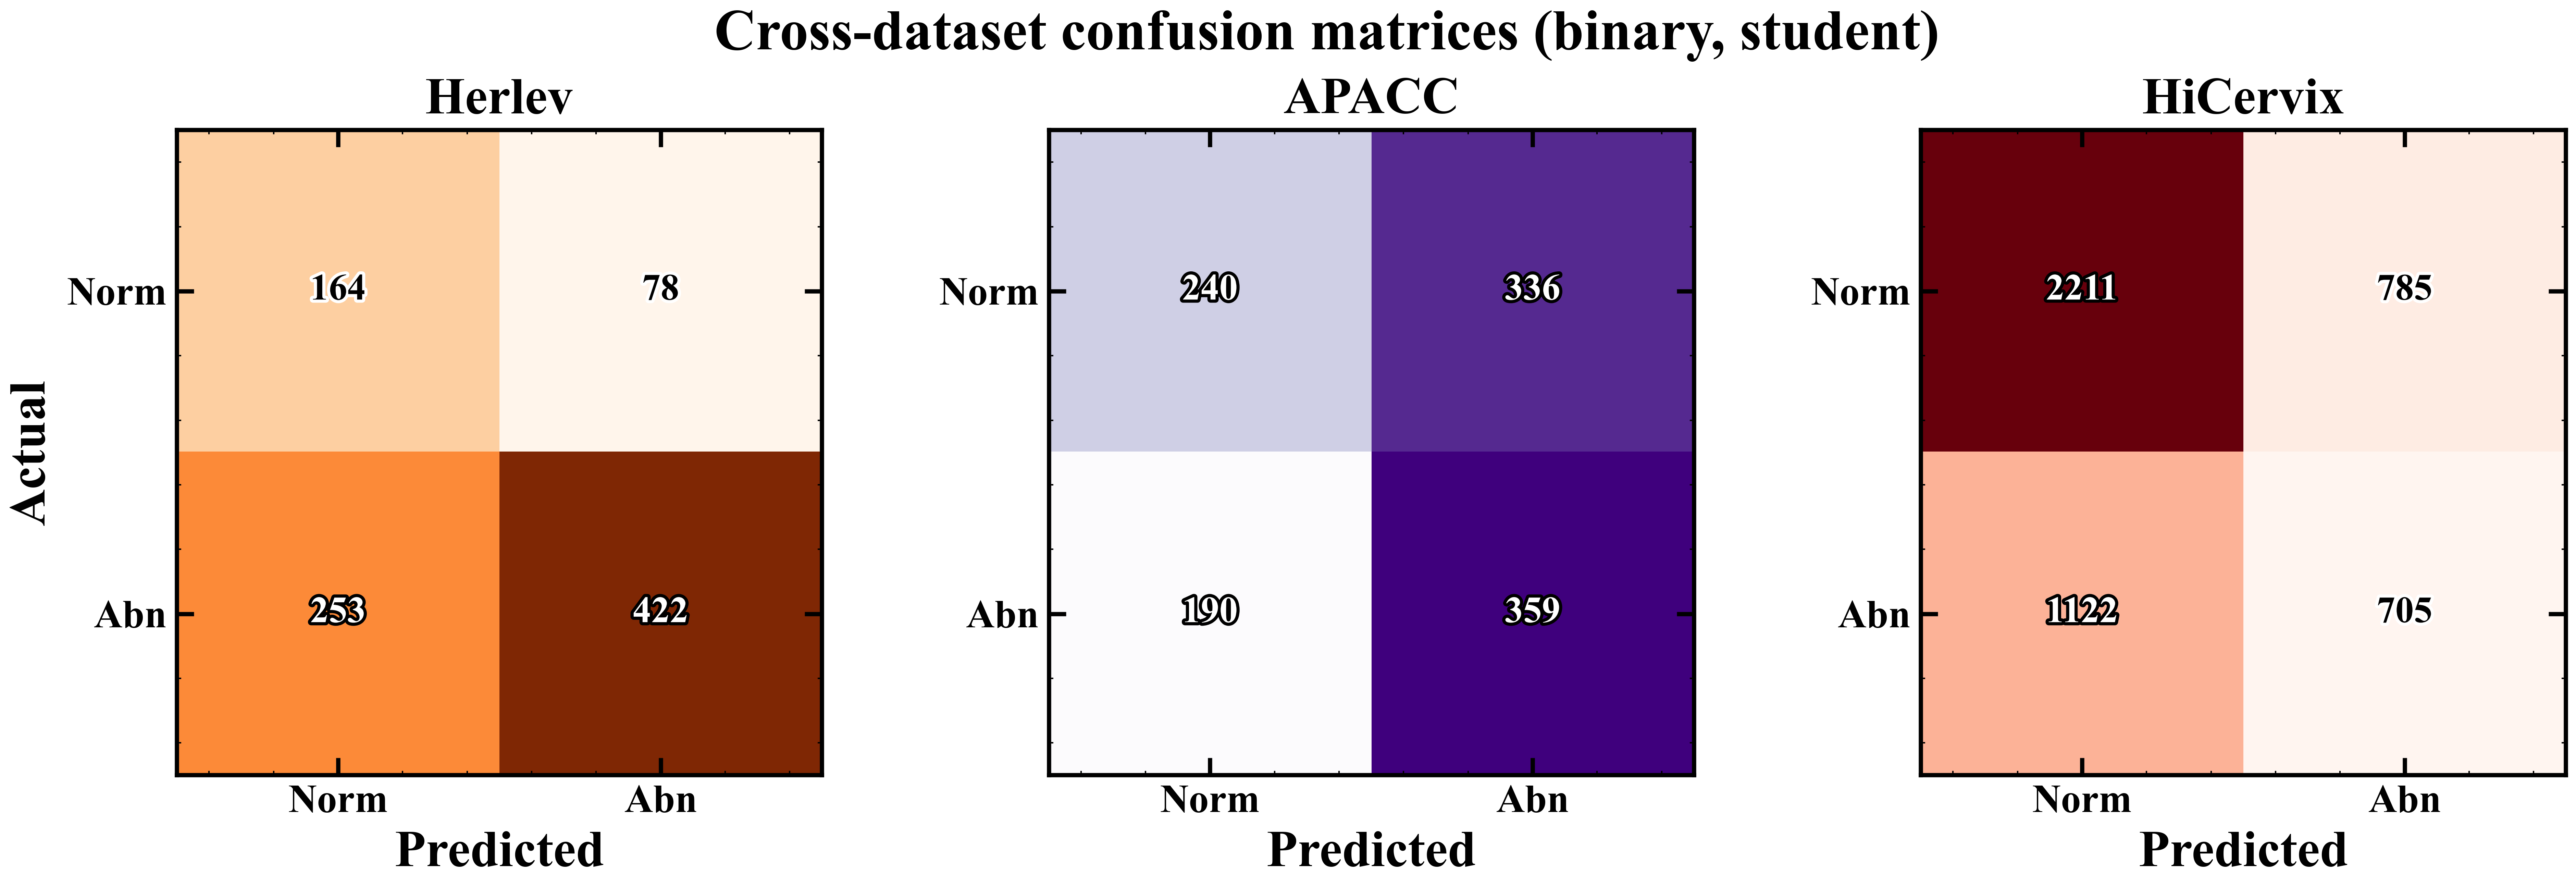
\includegraphics[width=\textwidth]{cm_cross_combined.png}
  \caption{Cross-dataset binary confusion matrices (student). The model over-predicts \emph{abnormal}
  on APACC (low specificity) and \emph{normal} on HiCervix (low sensitivity).}
  \label{fig:cmcross}
\end{figure*}

\section{Why cross-dataset evaluation fails}
\label{sec:why}
\textbf{(1) It is not a labelling artefact.} A flipped or mis-defined mapping would make the decision
score rank abnormal \emph{below} normal cells, giving AUROC$<0.5$. The opposite holds: the
separation $\Delta P$ between mean $P(\mathrm{abnormal})$ on true-abnormal and true-normal cells is
\emph{positive everywhere}---$+0.284$ (Herlev), $+0.112$ (HiCervix), $+0.045$ (APACC)---and every
AUROC exceeds $0.5$ (Figure~\ref{fig:sep}). The per-dataset mappers were audited explicitly
(Herlev $7\rightarrow$binary, APACC healthy/unhealthy, HiCervix Bethesda \texttt{level\_1}:
negative$\rightarrow$normal, ASC$\rightarrow$abnormal, AGC/microbe$\rightarrow$excluded). The labels
are correctly oriented; the model simply has little to rank with.

\begin{figure*}[t]
  \centering
  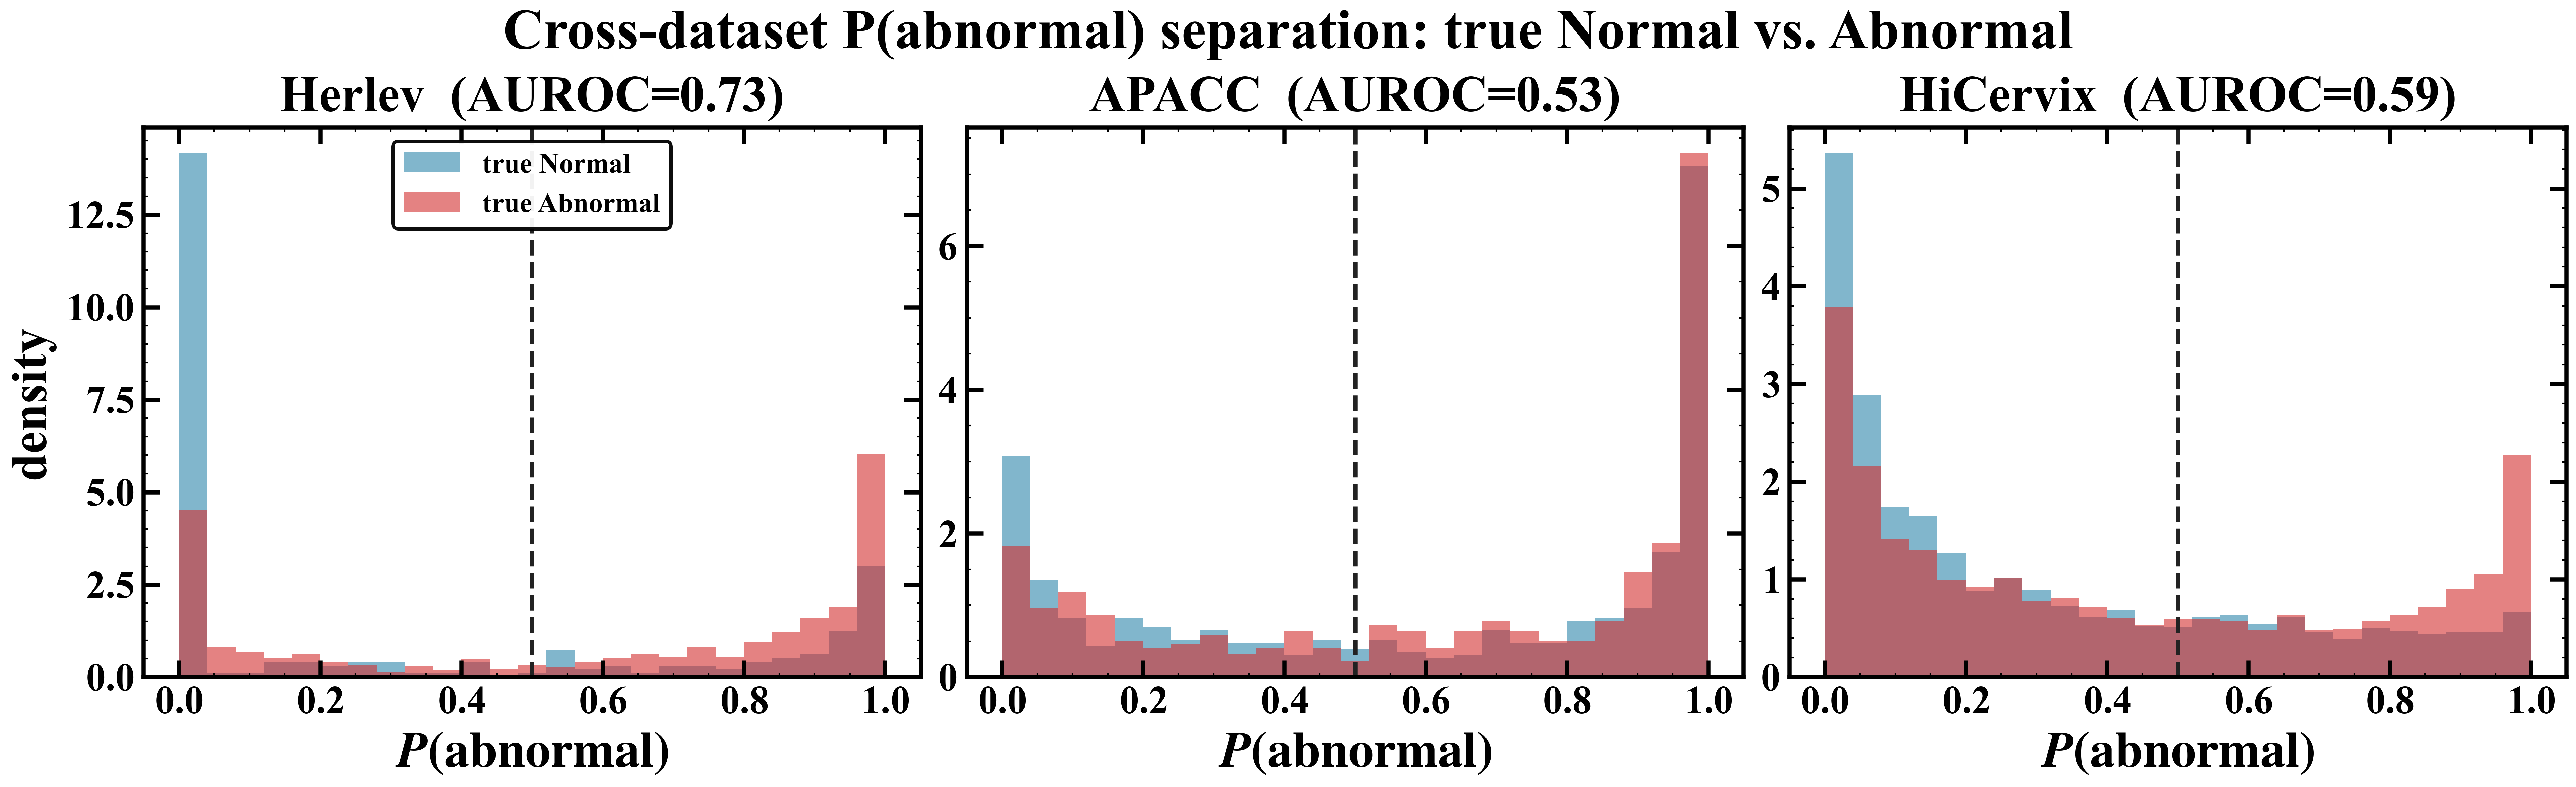
\includegraphics[width=\textwidth]{cross_separation.png}
  \caption{Distribution of the decision score $P(\mathrm{abnormal})$ for true-normal (blue) vs.\
  true-abnormal (red) cells. Separation is clear on Herlev (AUROC $0.73$), weak on HiCervix
  ($0.59$) and essentially absent on APACC ($0.53$). The dashed line is the $\tau{=}0.5$ threshold.}
  \label{fig:sep}
\end{figure*}

\textbf{(2) Operating-point miscalibration.} The well-calibrated in-distribution confidence does not
transfer: the $P(\mathrm{abnormal})$ distribution shifts per domain (baseline $\approx 0.6$ on APACC
$\rightarrow$ over-calls abnormal; $\approx 0.35$ on HiCervix $\rightarrow$ under-calls). At the
fixed $\tau{=}0.5$ the binary accuracy is therefore \emph{below the majority-class baseline} for both
Herlev ($0.639<0.74$) and HiCervix ($0.605<0.62$), even though the AUROC shows real ranking signal.
A per-domain optimal threshold recovers much of it (Herlev $0.75$ at $\tau{=}0.05$; HiCervix $0.65$
at $\tau{=}0.85$), but choosing $\tau$ on the test set is not an honest operating point---it only
quantifies the calibration gap.

\textbf{(3) The signal degrades with preparation distance.} The retained AUROC tracks how similar
each dataset's slide preparation is to SIPaKMeD's conventional smear: Herlev (conventional smear)
$0.73$ $>$ HiCervix (liquid-based) $0.59$ $>$ APACC (auto-segmented, noisy crops) $0.53\approx$
chance. The collapse is dominated by preparation/scanner/segmentation shift, exactly the axis a
single-source model is blind to.

\textbf{(4) The internal number is optimistic.} The $96.6\%$ is measured on a random per-cell
validation split, which leaks same field-of-view (FoV) cells across train and validation; a leakage-safe,
cluster-grouped split would lower it. The true internal$\rightarrow$external gap is therefore even
larger than the $\approx 33$-point drop observed here.

\section{Conclusion}
The audited model is internally excellent ($96.6\%$, well calibrated, cytologically faithful
Grad-CAM) yet \emph{does not generalize}: binary AUROC falls to $0.53$--$0.73$ across datasets and
binary accuracy drops below trivial baselines under a fixed threshold. Crucially, this is not a
labelling error---the decision score is correctly oriented in every dataset---but a combination of
domain-shift signal loss and operating-point miscalibration, on top of an optimistic leaky internal
estimate. Headline single-dataset accuracy is thus a poor proxy for screening readiness. The
indicated remedies are leakage-safe (cluster-grouped) evaluation, stain/domain
normalization~\citep{macenko2009stain} and per-domain calibration~\citep{guo2017calibration}, and
reporting threshold-free AUROC alongside the excluded fraction---not relabelling.

\bibliographystyle{unsrtnat}
\bibliography{references}

\end{document}
